\documentclass[11pt, a4paper]{article}

\usepackage{tikz}
\usetikzlibrary{arrows,automata, shapes, petri}
\usepackage{amsmath}

\begin{document}

\title{BACKPROPAGATION}
\date{}
\maketitle

Backpropagation is a computer algorithm used for supervised training of Artificial Neural Networks. It is based on two ideas - the Chain Rule of derivatives in Calculus and Dynamic Programming.

\section{Notation}

\begin{center}
	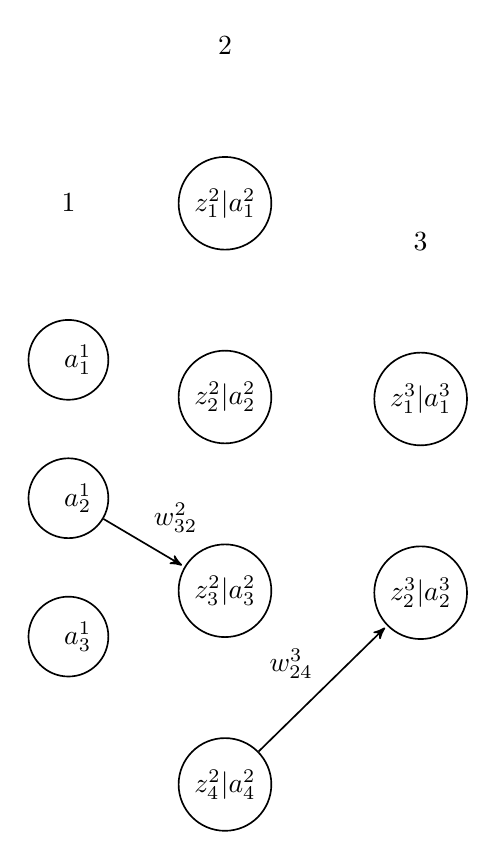
\begin{tikzpicture}[->,>=stealth',shorten >=1pt,auto,
		semithick]
														
		\node[state] (I1)                    {$\ \ a^1_1$};
		\node[state] (I2) [below of=I1, node distance=5em] {$\ \ a^1_2$};
		\node[state] (I3) [below of=I2, node distance=5em] {$\ \ a^1_3$};
						
		\node[state] (J1) [above right of=I1, node distance=8em]  {$z^2_1|a^2_1$};
		\node[state] (J2) [below of=J1, node distance=7em] {$z^2_2|a^2_2$};
		\node[state] (J3) [below of=J2, node distance=7em] {$z^2_3|a^2_3$};
		\node[state] (J4) [below of=J3, node distance=7em] {$z^2_4|a^2_4$};	
						
		\node[state] (K1) [below right of=J1, node distance=10em]  {$z^3_1|a^3_1$};
		\node[state] (K2) [below of=K1, node distance=7em] {$z^3_2|a^3_2$};	
						
		\node [rectangle, node distance=2cm] (I) [above of=I1] {1};
		\node [rectangle, node distance=2cm] (J) [above of=J1] {2};
		\node [rectangle, node distance=2cm] (K) [above of=K1] {3};	
						
		\path (I2) edge  node {$w^2_{32}$} (J3);	
		\path (J4) edge  node {$w^3_{24}$} (K2);		
						                   
	\end{tikzpicture}
\end{center}

The layers are of the Neural Network are denoted by positive integers with input layer denoted by $1$, the first hidden layer by $2$ and so on till the output layer. The inputs in the input layer are denoted by $a^1_{i}$ as shown above. For all the other neurons in other layers, $z^l_i$ denotes the weighted sum of the neuron activations in the previous layer and $a^l_i$ denotes that neuron's activation. The weights are superscripted by the index of the layer of the neuron at the end, and subscripted first by the layer index of the end neuron and then by that of the start neuron.

\section{Forward Pass}

For any layer $l$ which is apart from the input layer, it can be written,

\begin{align*}
	z^l_i = \left( \sum_j w^l_{ij}a^{l-1}_j \right)  + b^l_i 
\end{align*} 

Taking examples from the figure,

\begin{align*}
	z^2_1 = (w^2_{11}a^1_1  + w^2_{12}a^1_2  +  w^2_{13}a^1_3) + b^2_1 \\ 
	z^2_2 = (w^2_{21}a^1_1  + w^2_{22}a^1_2  +  w^2_{23}a^1_3) + b^2_2 \\
	z^2_3 = (w^2_{31}a^1_1  + w^2_{32}a^1_2  +  w^2_{33}a^1_3) + b^2_3 \\
	z^2_4 = (w^2_{41}a^1_1  + w^2_{42}a^1_2  +  w^2_{43}a^1_3) + b^2_4 
\end{align*}

These equations can be rewritten in matrix form as follows,

\begin{align*}
	\begin{pmatrix} z^2_1 \\ z^2_2 \\ z^2_3 \\z^2_4 \end{pmatrix} = \begin{pmatrix}  w^2_{11} & w^2_{12} & w^2_{13} \\ w^2_{21} & w^2_{22} & w^2_{23} \\ w^2_{31} & w^2_{32} & w^2_{33} \\w^2_{41} & w^2_{42} & w^2_{43}  \end{pmatrix} \begin{pmatrix} a^1_1 \\ a^1_2 \\ a^1_3 \\ \end{pmatrix} + \begin{pmatrix} b^2_1 \\ b^2_2 \\ b^2_3 \\b^2_4 \end{pmatrix}	
\end{align*}

or 

\begin{align*}
	\boldsymbol{Z}^2 = \boldsymbol{W}^2 \boldsymbol{A}^1 + \boldsymbol{B}^2 
\end{align*}

Generalizing for all layers,

\begin{align}
	\boldsymbol{Z}^l = \boldsymbol{W}^l \boldsymbol{A}^{l-1} + \boldsymbol{B}^l 
\end{align}

Activation function $\sigma$ is applied to $z^l_i$ to yield $a^l_i$.

\begin{align*}
	a^2_1 = \sigma(z^2_1) \\
	a^2_2 = \sigma(z^2_2) \\
	a^2_3 = \sigma(z^2_3) \\
	a^2_4 = \sigma(z^2_4) \\
\end{align*} 

which can be written in matrix form as,

\begin{align*}
	\boldsymbol{Z}^2 = \sigma(\boldsymbol{A}^2) 
\end{align*}

or more generally as,

\begin{align}
	\boldsymbol{Z}^l = \sigma(\boldsymbol{A}^l) 
\end{align}

Given $\boldsymbol{A}^1$, any $\boldsymbol{Z}^l$ or $\boldsymbol{A}^l$ can be calculated using the two equations (1) and (2). This completes the analysis of the forward pass of backpropagation algorithm.

\section{Backward Pass}

Imagine a point in time where the weights and biases of a neural network are fixed. Now, one training example is taken and its inputs are fed into the neural network. Using the the forward pass equations, the neural network's output is computed. Usually, this output is different from the training example's expected output and thus the goal of backpropagation is to calucate the partial derivates of the cost function w.r.t. each weight and bias for them to be tweaked optimally.

\subsection{Cost Function}

The notion of the difference between the expected output of a training example and the actual output from neural network is formalized as follows,

\begin{align*}
	C & = \frac{1}{2} ||\boldsymbol{Y} - \boldsymbol{A}^L||^2 \\
	  & = \frac{1}{2}\sum_j (y_j - a^L_j)^2                   
\end{align*}

\subsection {Backpropagation}

\begin{align*}
	\frac{\partial C}{\partial z^L_j} & = (a^L_j - y_j) \frac{\partial a^L_j}{\partial z^L_j} \\
	                                  & = (a^L_j - y_j) \times \sigma^{'} (z^L_j)             
\end{align*}

Denoting $\frac{\partial C}{\partial z^L_j}$ by $\delta^L_j$ and $(\delta^L_1, \delta^L_2, .. )^T$ by $\boldsymbol{\Delta^L}$, it can be written

\begin{align}
	\boldsymbol{\Delta^L} = (\boldsymbol{A^L} - \boldsymbol{Y}) \odot \sigma^{'}(\boldsymbol{Z^L}) 
\end{align}

where $\odot$ denotes element-wise matrix product.

Can $\boldsymbol{\Delta^L}$ somehow be related to $\boldsymbol{\Delta^{L-1}}$?

\begin{align*}
	\delta^{L-1}_j & = \frac{\partial C}{\partial z^{L-1}_j}                                                                                              \\
	               & = \frac{\partial C}{\partial a^{L-1}_j} \frac{\partial a^{L-1}_j}{\partial z^{L-1}_j}                                                \\
	               & = \frac{\partial C}{\partial a^{L-1}_j} \times \sigma^{'}(z^{L-1}_j)                                                                 \\
	               & = \left( \sum_i \frac{\partial z^{L}_i}{\partial a^{L-1}_j} \frac{\partial C}{\partial z^{L}_i} \right) \times \sigma^{'}(z^{L-1}_j) \\
	               & = \left( \sum_i w^L_{ij} \delta^L_i \right) \times \sigma^{'}(z^{L-1}_j)                                                             \\
\end{align*}

For the above example, the equations become

\begin{align*}
	\begin{pmatrix} \delta^{L-1}_1 \\ \delta^{L-1}_2 \\ \delta^{L-1}_3 \\ \delta^{L-1}_4 \end{pmatrix} &= \begin{pmatrix}  w^L_{11} & w^L_{21} \\ w^L_{12} & w^L_{22} \\ w^L_{13} & w^L_{23} \\w^L_{14} & w^L_{24}  \end{pmatrix} \begin{pmatrix} \delta^L_1 \\ \delta^L_2 \end{pmatrix} \odot \begin{pmatrix} \sigma^{'}(z^{L-1}_1) \\ \sigma^{'}(z^{L-1}_2) \\ \sigma^{'}(z^{L-1}_3) \\ \sigma^{'}(z^{L-1}_4) \end{pmatrix} \\		
	\boldsymbol{\Delta^{L-1}} &= \boldsymbol{W^L}^T \boldsymbol{\Delta^L} \odot \sigma^{'}(\boldsymbol{Z^{L-1}})
\end{align*}

The equation can be generalized to,

\begin{align}
	\boldsymbol{\Delta^{l}} & = \boldsymbol{W^{l+1}}^T \boldsymbol{\Delta^{l+1}} \odot \sigma^{'}(\boldsymbol{Z^{l}}) 
\end{align}

Using equation (3) and (4) $\boldsymbol{\Delta^{l}}$ can be calculated for any $l$.

\begin{align}
	\frac{\partial C}{\partial w^l_{jk}} & = \frac{\partial z^l_{j}}{\partial w^l_{jk}} \frac{\partial C}{\partial z^l_{j}}             
	= a^{l-1}_k \delta^l_j \\
	\frac{\partial C}{\partial b^l_{j}}  & = \frac{\partial z^l_{j}}{\partial b^l_{j}} \frac{\partial C}{\partial z^l_{j}} = \delta^l_j 
\end{align}

Hence, equations (3) and (4) ``propagate" the error backwards and then with help of equations (5) and (6), partial derivative of the error w.r.t. any neural network weight or bias can be calculated.

\section{Conclusion}

Backpropagation is famous because it can quickly calculate partial derivatives to optimally adjust the parameters of a neural network. In the description above, backpropagation calculates the derivatives w.r.t only one training example. In practice training examples are bunched into mini-batches and partials calculated for each example in a mini batch are averaged for network parameter adjustment.

\end{document}